%NO MODIFICAR ESTA SECCION!
\documentclass{article} % Define la clase del documento, en este caso, un artículo

\usepackage[letterpaper,margin=3cm]{geometry} % Configura el tamaño del papel y los márgenes del documento
\usepackage{graphicx} % Permite la inserción de imágenes
\usepackage[spanish]{babel}% Activar esta configuración para informes en español, ajusta el idioma del documento
\usepackage[usenames]{color} % Permite el uso de colores definidos por nombre en el documento
\usepackage{hyperref} % Habilita enlaces y referencias dentro del documento
\hypersetup{colorlinks=true, linkcolor = black, citecolor= black} % Configura el color de los enlaces y citas
\usepackage{booktabs} % Proporciona comandos para crear tablas de alta calidad
\usepackage{natbib} % Permite el uso de citas y referencias bibliográficas con diferentes estilos
\usepackage{tikz} % Permite la creación de gráficos y diagramas vectoriales directamente en LaTeX
\usepackage{float} % Para controlar la posición de los elementos flotantes, como imágenes, con la opción [H]
\bibliographystyle{agsm} % Define el estilo de citas y bibliografía (en este caso, el estilo AGSM)
\usepackage{diagbox} % Permite crear celdas con líneas diagonales en tablas
\usepackage{listings} % Permite la inclusión y formateo de código fuente en el documento
\usepackage{xcolor} % Paquete para definir y usar colores en el documento
\usepackage{parskip} % Añade espacio entre párrafos en lugar de sangrías
\usepackage{fancyhdr} % Permite personalizar encabezados y pies de página
\usepackage{amsmath} % Proporciona una amplia variedad de entornos y comandos matemáticos
\usepackage{enumitem}
\usepackage{tcolorbox}

% Definimos colores
\definecolor{levelone}{RGB}{230, 230, 250}   % lavanda claro
\definecolor{leveltwo}{RGB}{255, 228, 225}   % rosa claro
\definecolor{levelthree}{RGB}{224, 255, 255} % cian claro
\definecolor{levelfour}{RGB}{240, 255, 240}  % verde claro

\newtcolorbox{highlightbox}[1][]{colback=#1, colframe=white, boxrule=0pt, arc=0pt, left=2pt, right=2pt, top=2pt, bottom=2pt}

\pagestyle{fancy} % Usa el estilo fancyhdr
\fancyhf{} % Borra todos los encabezados y pies de página
\renewcommand{\headrulewidth}{0pt}
\renewcommand{\footrulewidth}{0pt} % Desactiva la línea horizontal predeterminada en el pie
\setlength{\headheight}{2cm} % Ajusta la altura del encabezado para hacer espacio para la línea
\fancyhead[L]{\raisebox{0.20cm}{\textbf{Fluid Mechanics}}} % Añade el texto en la parte izquierda del encabezado, subiéndolo ligeramente
\fancyhead[R]{\raisebox{0.1cm}{
\includegraphics[width=0.25\linewidth]{LOGO_UNIVERSIDAD.jpg}}} % Añade la imagen en la parte derecha del encabezado y súbela un poco
\fancyhead[C]{\rule{\textwidth}{0.6pt}} % Añade una línea horizontal superior centrada
\fancyfoot[C]{\rule{\textwidth}{0.6pt}} % Añade una línea horizontal en el pie de página centrada
\fancyfoot[R]{\raisebox{-1.5\baselineskip}{\thepage}} % Coloca el número de página a la derecha, con suficiente espacio debajo de la línea
\geometry{top=3cm, bottom=2.5cm} % Ajusta los márgenes superior e inferior

% Definición de colores al estilo Visual Studio Code
\definecolor{codegreen}{rgb}{0.25,0.49,0.48} % Comentarios
\definecolor{codegray}{rgb}{0.5,0.5,0.5} % Números y anotaciones
\definecolor{codepurple}{rgb}{0.58,0,0.82} % Palabras clave
\definecolor{backcolour}{rgb}{0.95,0.95,0.92} % Color de fondo

% Configuración del estilo de las celdas de código
\lstset{
    backgroundcolor=\color{backcolour},   % color de fondo; necesita que el paquete color o xcolor esté cargado
    commentstyle=\color{codegreen},       % estilo de comentarios
    keywordstyle=\color{codepurple},      % estilo de palabras clave
    numberstyle=\tiny\color{codegray},    % estilo de los números de línea
    stringstyle=\color{red},              % estilo de las cadenas de texto
    basicstyle=\ttfamily\small,           % estilo del texto básico
    breakatwhitespace=false,              % ajustes de líneas sólo en espacios en blanco
    breaklines=true,                      % ajustar las líneas si son muy largas
    captionpos=b,                         % posición de la leyenda (abajo)
    keepspaces=true,                      % preserva los espacios en el texto; útil si se usa monoespaciado
    numbers=left,                         % dónde poner los números de línea
    numbersep=5pt,                        % qué tan lejos están los números de línea del código
    showspaces=false,                     % mostrar espacios con subrayados particulares; reemplaza 'showstringspaces'
    showstringspaces=false,               % subrayar los espacios dentro de las cadenas solo
    showtabs=false,                       % mostrar tabulaciones en el código con subrayados particulares
    tabsize=2,                            % tamaños de tabulación a 2 espacios
    language=TeX,                         % lenguaje del código
    morecomment=[l]\#,                    % reconocer # como inicio de comentario en Python
    frame=single,                         % agregar un marco simple alrededor del código
    rulecolor=\color{black}               % color del marco
}

\begin{document}
%----------------------------------------------------------------------------------------
%   PORTADA
%Modificar desde aqui en adelante
%----------------------------------------------------------------------------------------
\begin{titlepage}%Inicio de la carátula, solo modificar los datos necesarios
\newcommand{\HRule}{\rule{\linewidth}{0.5mm}} 
\center 
%----------------------------------------------------------------------------------------
%	ENCABEZADO
%----------------------------------------------------------------------------------------

\includegraphics[width=10cm]{LOGO_UNIVERSIDAD.jpg}\\ % Si esta plantilla se copio correctamente, va a llevar la imagen del logo de la facultad.OBS: Es necesario incluir el paquete: graphicx
\vspace{3cm}
%----------------------------------------------------------------------------------------
%	SECCION DEL TITULO
%----------------------------------------------------------------------------------------
\HRule \\[0.4cm]
{ \huge \bfseries Tittle}\\[0.4cm] % Titulo del documento
{ \huge \bfseries Fluid Mechanics}\\[0.4cm] % Titulo del documento
\HRule \\[1.5cm]
 \vspace{5cm}
%----------------------------------------------------------------------------------------
%	SECCION DEL AUTOR
%----------------------------------------------------------------------------------------
\begin{flushright}
    { \textbf{Profesors:}\\
    Patricio Moreno\\
    Sebastian Sepulveda\\
    \vspace{0.2cm}
    \textbf{Assistant:}\\
    Lukas Wolff\\
    \vspace{0.2cm}
    \textbf{Author:}\\
    Pepe\\
}
\end{flushright}
\vspace{1cm}
%----------------------------------------------------------------------------------------
%	SECCION DE LA FECHA
%----------------------------------------------------------------------------------------
{\large \textbf{\today}}\\[2cm] % El comando \today coloca la fecha del dia, y esto se actualiza con cada compilacion, en caso de querer tener una fecha estatica, reemplazar el \today por la fecha deseada
\end{titlepage}
%----------------------------------------------------------------------------------------
%  INDICE
%----------------------------------------------------------------------------------------
\newpage
\tableofcontents
\thispagestyle{plain} % Deshabilita el encabezado en la página del índice
\thispagestyle{empty} % Deshabilita el número de página en la página del índice
\newpage

%Se puede agregar un indice de figuras si es nesesario
%\newpage
%\listoffigures 
%\thispagestyle{plain} % Deshabilita el encabezado en la página del índice %
%\thispagestyle{empty}
%\newpage
%----------------------------------------------------------------------------------------
%   ACÁ EMPIEZA EL INFORME
\setcounter{page}{1} % Reinicia el contador de páginas
%----------------------------------------------------------------------------------------
%Este es el formato a seguir para los titulos de las secciones
\section{Capitulo 1}

\subsection{Proyecto}

\begin{itemize}[label={},left=0pt,align=parleft]
    \item \begin{highlightbox}[levelone] Es un conjunto de actividades relacionadas entre sí \end{highlightbox}
    \item \begin{highlightbox}[levelone] Los proyectos son únicos \end{highlightbox}
    \item \begin{highlightbox}[levelone] Relaciona un equipo de trabajo, en un periodo de tiempo bajo requisitos específicos \end{highlightbox}
\end{itemize}

\subsection{Tipos de Proyectos}

\begin{itemize}[label={},left=0pt,align=parleft]
    \item \begin{highlightbox}[levelone] Proyectos de Construcción \end{highlightbox}
    \begin{itemize}[label={},left=1em,align=parleft]
        \item \begin{highlightbox}[leveltwo] Es un tipo de proyecto que tiene asignados objetivos, especificaciones, plazo y presupuesto \end{highlightbox}
        \item \begin{highlightbox}[leveltwo] Tipos de construcciones: \end{highlightbox}
        \begin{itemize}[label={},left=2em,align=parleft]
            \item \begin{highlightbox}[levelthree] Habitacional \end{highlightbox}
            \item \begin{highlightbox}[levelthree] No habitacional \end{highlightbox}
            \item \begin{highlightbox}[levelthree] Industrial \end{highlightbox}
            \item \begin{highlightbox}[levelthree] Obras Civiles \end{highlightbox}
        \end{itemize}
        \item \begin{highlightbox}[leveltwo] Tipos de Vida: \end{highlightbox}
        \begin{itemize}[label={},left=2em,align=parleft]
            \item \begin{highlightbox}[levelthree] Vida de Diseño: Es la vista prevista del proyecto, es la que se espera que tenga. \end{highlightbox}
            \item \begin{highlightbox}[levelthree] Vida Útil: Es la duración estimada que un objeto debe tener, respecto a factores externos. \end{highlightbox}
            \item \begin{highlightbox}[levelthree] Vida Remanente: Es el periodo durante el cual un objeto puede utilizarse de forma rentable antes de que la mantención ya no sea viable. \end{highlightbox}
        \end{itemize}
        \item \begin{highlightbox}[leveltwo] Etapas de un Proyecto de Construcción: \end{highlightbox}
        \begin{itemize}[label={},left=2em,align=parleft]
            \item \begin{highlightbox}[levelthree] Existe una necesidad \end{highlightbox}
            \item \begin{highlightbox}[levelthree] Análisis \end{highlightbox}
            \item \begin{highlightbox}[levelthree] Identificación de soluciones \end{highlightbox}
            \item \begin{highlightbox}[levelthree] Estudios de Factibilidad \end{highlightbox}
            \item \begin{highlightbox}[levelthree] Evaluación \end{highlightbox}
            \item \begin{highlightbox}[levelthree] Financiamiento \end{highlightbox}
            \item \begin{highlightbox}[levelthree] Diseño, que considera los siguientes aspectos: \end{highlightbox}
            \begin{itemize}[label={},left=3em,align=parleft]
                \item \begin{highlightbox}[levelfour] Estudio de Terreno \end{highlightbox}
                \item \begin{highlightbox}[levelfour] Diseño Arquitectónico \end{highlightbox}
                \item \begin{highlightbox}[levelfour] Diseño Estructural \end{highlightbox}
                \item \begin{highlightbox}[levelfour] Estudios de Impacto Ambiental \end{highlightbox}
                \item \begin{highlightbox}[levelfour] Diseño de Instalaciones \end{highlightbox}
                \item \begin{highlightbox}[levelfour] Redacción de documentos de licitación \end{highlightbox}
                \item \begin{highlightbox}[levelfour] Constructibilidad y Mantención \end{highlightbox}
            \end{itemize}
            \item \begin{highlightbox}[levelthree] Licitacion \end{highlightbox}
            \item \begin{highlightbox}[levelthree] Construcción \end{highlightbox}
            \item \begin{highlightbox}[levelthree] Puesta en Marcha \end{highlightbox}
        \end{itemize}
    \end{itemize}
\end{itemize}

De esta manera, un proyecto de construcción se puede expresar de la siguiente manera:

\begin{figure}[H]
    \centering
    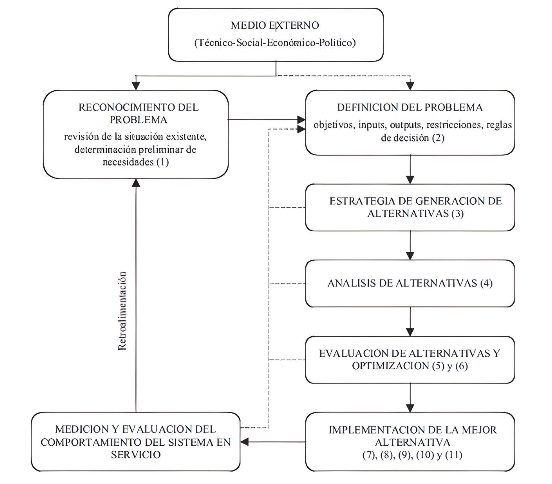
\includegraphics[width=0.5\textwidth]{proyecto_construccion.png}
    \caption{Proyecto de Construcción}
    \label{fig:ProyectoConstruccion}
\end{figure}

\section{Capítulo 2}

\subsection{Diseño de un Proyecto de Construcción}

\begin{itemize}[label={},left=0pt,align=parleft]
    \item \begin{highlightbox}[levelone] Estudio de terreno, el cual consta de: \end{highlightbox}
    \begin{itemize}[label={},left=1em,align=parleft]
        \item \begin{highlightbox}[leveltwo] Ubicación del terreno \end{highlightbox}
        \item \begin{highlightbox}[leveltwo] Condiciones propias tales como: \end{highlightbox}
        \begin{itemize}[label={},left=2em,align=parleft]
            \item \begin{highlightbox}[levelthree] Topografía \end{highlightbox}
            \item \begin{highlightbox}[levelthree] Geología \end{highlightbox}
            \item \begin{highlightbox}[levelthree] Hidrología \end{highlightbox}
            \item \begin{highlightbox}[levelthree] Fuentes de Abastecimiento como energía y comunicaciones \end{highlightbox}
        \end{itemize}
        \item \begin{highlightbox}[leveltwo] Aspectos Legales, específicos a cada zona. \end{highlightbox}
        \item \begin{highlightbox}[leveltwo] Condiciones de servicio, como agua potable, electricidad o alcantarillado. \end{highlightbox}
        \item \begin{highlightbox}[leveltwo] Evaluación de impacto ambiental. \end{highlightbox}
    \end{itemize}
\end{itemize}

\subsection{Leyes}

\begin{itemize}[label={},left=0pt,align=parleft]
    \item \begin{highlightbox}[levelone] Ley general de urbanismo y construcciones (DFL 458, MINVU): Contiene el proceso global de urbanismo y construcción. \end{highlightbox}
    \item \begin{highlightbox}[levelone] Ley Base del Medio Ambiente (Ley 19.300): Regula el derecho a vivir en un medio ambiente libre de contaminación. \end{highlightbox}
    \item \begin{highlightbox}[levelone] Ley para la construcción de viviendas económicas (DFL-2 de 1959): Desarrollo el concepto de vivienda económica como aquella que tiene max 140 $m^2$ y no excede los 17.5 $m^2$ edificados por cama. \end{highlightbox}
    \item \begin{highlightbox}[levelone] Decreto Ley 2552-1979: Busca resolver los problemas de marginalidad habitacional, también define el concepto de vivienda de emergencia. \end{highlightbox}
    \item \begin{highlightbox}[levelone] Código del Trabajo (2002): Regula remuneraciones, gratificaciones, contratos, descansos, etc. \end{highlightbox}
    \item \begin{highlightbox}[levelone] Ley sobre accidente de trabajo y enfermedades profesionales (16.744): Establece un seguro obligatorio contra accidentes del trabajo y enfermedades profesionales. \end{highlightbox}
    \item \begin{highlightbox}[levelone] Ley de subcontratación (20.123): Regula la subcontratación de trabajadores. \end{highlightbox}
    \item \begin{highlightbox}[levelone] Ley de Concesiones (DFL 164) y Reglamento (DS 240) de Concesiones de Obras Públicas: Regula la concesión de obras públicas. \end{highlightbox}
    \item \begin{highlightbox}[levelone] Código Civil: El constructor tiene una responsabilidad de 5 años sobre la obra. \end{highlightbox}
    \item \begin{highlightbox}[levelone] Ley de la venta por piso o ley de propiedad horizontal (Ley 6071): Regula la venta de departamentos en construcción. \end{highlightbox}
    \item \begin{highlightbox}[levelone] Ley que incorpora el IVA a las empresas constructoras (Ley 18.630). \end{highlightbox}
    \item \begin{highlightbox}[levelone] etc. \end{highlightbox}
\end{itemize}

\subsection{Normas}

INN $=>$ Instituto Nacional de Normalización, cumplir sus normas no es de carácter obligatorio. Algunas de las áreas que cubre:

\begin{itemize}[label={},left=0pt,align=parleft]
    \item \begin{highlightbox}[levelone] General \end{highlightbox}
    \item \begin{highlightbox}[levelone] Diseño Arquitectónico \end{highlightbox}
    \item \begin{highlightbox}[levelone] Diseño, Cálculo y Ejecución de Estructuras \end{highlightbox}
    \item \begin{highlightbox}[levelone] Acondicionamiento Ambiental \end{highlightbox}
    \item \begin{highlightbox}[levelone] Materiales y Componentes \end{highlightbox}
    \item \begin{highlightbox}[levelone] Instalaciones \end{highlightbox}
    \item \begin{highlightbox}[levelone] Herramientas \end{highlightbox}
\end{itemize}

\subsection{Especificaciones Técnicas}

Corresponden a documentos asociados al proyecto, y sirven como complemento hacia los planos.

\subsection{Permisos y derechos de Construcción}

Las obras privadas deben tener un permiso de construcción, antes de comenzar su ejecución.

\subsection{Permisos de Construcción}

Se solicita a la dirección de obras municipales, para su obtención, se debe seguir el siguiente proceso:

\begin{itemize}[label={},left=0pt,align=parleft]
    \item \begin{highlightbox}[levelone] Solicitud de permiso: firmada por el propietario y arquitecto del proyecto \end{highlightbox}
    \item \begin{highlightbox}[levelone] Legado de documentos, que incluye: \end{highlightbox}
    \begin{itemize}[label={},left=1em,align=parleft]
        \item \begin{highlightbox}[leveltwo] Fotocopia de certificado y informaciones previas. \end{highlightbox}
        \item \begin{highlightbox}[leveltwo] Formulario único de estadísticas de edificación. \end{highlightbox}
        \item \begin{highlightbox}[leveltwo] Certificado de factibilidad de servicios \end{highlightbox}
        \item \begin{highlightbox}[leveltwo] Planos de Arquitectura \end{highlightbox}
        \item \begin{highlightbox}[leveltwo] Proyecto de cálculo estructural \end{highlightbox}
        \item \begin{highlightbox}[leveltwo] Cuadros de superficie \end{highlightbox}
        \item \begin{highlightbox}[leveltwo] Especificaciones técnicas de las partidas \end{highlightbox}
        \item \begin{highlightbox}[leveltwo] Levantamiento topográfico \end{highlightbox}
    \end{itemize}
    \item \begin{highlightbox}[levelone] Pago de derechos municipales \end{highlightbox}
    \item \begin{highlightbox}[levelone] Firma de documentos \end{highlightbox}
\end{itemize}

\subsection{Sistema de Evaluación de Impacto Ambiental SEIA}

Se establece que toda persona tiene derecho a vivir en un ambiente libre de contaminación. El SEIA es un instrumento de carácter preventivo, donde se determina si un proyecto se ajusta a las normas ambientales vigentes.

Los siguientes proyectos deben someterse a SEIA:

\begin{itemize}[label={},left=0pt,align=parleft]
    \item \begin{highlightbox}[levelone] Acueductos, embalses o tranques \end{highlightbox}
    \item \begin{highlightbox}[levelone] Líneas de transmisión eléctrica de alto voltaje \end{highlightbox}
    \item \begin{highlightbox}[levelone] Aeropuertos, terminales de buses, camiones y trenes \end{highlightbox}
    \item \begin{highlightbox}[levelone] Proyectos de desarrollo urbano y turístico \end{highlightbox}
    \item \begin{highlightbox}[levelone] Instalaciones fabriles \end{highlightbox}
    \item \begin{highlightbox}[levelone] Agroindustrias \end{highlightbox}
    \item \begin{highlightbox}[levelone] Proyectos de explotación forestal \end{highlightbox}
    \item \begin{highlightbox}[levelone] Proyectos que conllevan el uso de sustancias tóxicas \end{highlightbox}
    \item \begin{highlightbox}[levelone] Proyectos de saneamiento ambiental \end{highlightbox}
    \item \begin{highlightbox}[levelone] Ejecución de obras en parques nacionales \end{highlightbox}
\end{itemize}

Documentos que deben presentarse:

\begin{itemize}[label={},left=0pt,align=parleft]
    \item \begin{highlightbox}[levelone] Descripción del proyecto \end{highlightbox}
    \item \begin{highlightbox}[levelone] Un plan de cumplimiento de legislación vigente \end{highlightbox}
    \item \begin{highlightbox}[levelone] Razones que hacen necesaria el EIA y no DIA \end{highlightbox}
    \item \begin{highlightbox}[levelone] Condiciones ambientales previas al proyecto \end{highlightbox}
    \item \begin{highlightbox}[levelone] Predicción de los impactos ambientales por el proyecto \end{highlightbox}
    \item \begin{highlightbox}[levelone] Medidas que se tomarán para eliminar o disminuir los impactos \end{highlightbox}
    \item \begin{highlightbox}[levelone] Acciones previas al estudio \end{highlightbox}
\end{itemize}

\subsubsection{Estudio de Impacto Ambiental (EIA)}

Es un conjunto de estudios necesarios para evaluar el impacto ambiental de un proyecto. Se debe presentar un EIA cuando un proyecto presenta uno de los siguientes impactos:

\begin{itemize}[label={},left=0pt,align=parleft]
    \item \begin{highlightbox}[levelone] Riesgosa para la salud de la población \end{highlightbox}
    \item \begin{highlightbox}[levelone] Efectos adversos sobre recursos naturales renovables \end{highlightbox}
    \item \begin{highlightbox}[levelone] Alteración de comunidades en los sistemas de vida \end{highlightbox}
    \item \begin{highlightbox}[levelone] Localización próxima a poblaciones \end{highlightbox}
    \item \begin{highlightbox}[levelone] Recursos o áreas protegidas \end{highlightbox}
    \item \begin{highlightbox}[levelone] Alteración significativa del valor paisajístico y/o turístico de la zona \end{highlightbox}
    \item \begin{highlightbox}[levelone] Alteración de monumentos \end{highlightbox}
\end{itemize}

\subsubsection{Declaración de Impacto Ambiental (DIA)}

Si un proyecto no presenta alguno de los impactos anteriores, solo debe presentar una declaración de impacto ambiental (DIA). Debe explicar por qué no es necesario el EIA, declarando sus compromisos ambientales. \\ \\
La principal diferencia entre un EIA y una DIA es que el EIA es un estudio más profundo y detallado, mientras que la DIA es un estudio más superficial. \\ \\
El DIA se rechaza si:

\begin{itemize}[label={},left=0pt,align=parleft]
    \item \begin{highlightbox}[levelone] No cumple la normativa \end{highlightbox}
    \item \begin{highlightbox}[levelone] No se subsanan los errores, omisiones o inexactitudes de ella \end{highlightbox}
    \item \begin{highlightbox}[levelone] El respectivo proyecto o actividad requiere de un EIA \end{highlightbox}
\end{itemize}

\subsection{Participantes de un proyecto de construcción}

\begin{itemize}[label={},left=0pt,align=parleft]
    \item \begin{highlightbox}[levelone] Durante el estudio y diseño: \end{highlightbox}
    \begin{itemize}[label={},left=1em,align=parleft]
        \item \begin{highlightbox}[leveltwo] Consultores Financieros \end{highlightbox}
        \item \begin{highlightbox}[leveltwo] Arquitectos \end{highlightbox}
        \item \begin{highlightbox}[leveltwo] Ingenieros \end{highlightbox}
        \item \begin{highlightbox}[leveltwo] Asesores Legales, Ambientales y de Construcción \end{highlightbox}
        \item \begin{highlightbox}[leveltwo] Otros \end{highlightbox}
    \end{itemize}
    \item \begin{highlightbox}[levelone] Durante la construcción: \end{highlightbox}
    \begin{itemize}[label={},left=1em,align=parleft]
        \item \begin{highlightbox}[leveltwo] Empresas constructoras \end{highlightbox}
        \item \begin{highlightbox}[leveltwo] Subcontratistas \end{highlightbox}
        \item \begin{highlightbox}[leveltwo] Inspección técnica de la obra (ITO) \end{highlightbox}
        \item \begin{highlightbox}[leveltwo] Organismos reguladores \end{highlightbox}
        \item \begin{highlightbox}[leveltwo] Proveedores \end{highlightbox}
        \item \begin{highlightbox}[leveltwo] Laboratorios de control de calidad \end{highlightbox}
        \item \begin{highlightbox}[leveltwo] Abogados \end{highlightbox}
        \item \begin{highlightbox}[leveltwo] Entidades de seguros \end{highlightbox}
        \item \begin{highlightbox}[leveltwo] Entidades ambientales \end{highlightbox}
        \item \begin{highlightbox}[leveltwo] Auditores bancarios \end{highlightbox}
        \item \begin{highlightbox}[leveltwo] Visitadores de obras \end{highlightbox}
        \item \begin{highlightbox}[leveltwo] Otros \end{highlightbox}
    \end{itemize}
\end{itemize}

\section{Capítulo 4: Contratos y propuestas en proyectos de Construcción}

Es un convenio entre el que construye y el dueño o mandante que financia, y fija sus objetivos
de acuerdo con sus necesidades y posibilidades. El propósito de un contrato de construcción
es definir derechos, obligaciones y responsabilidades de cada una de las partes involucradas.
\\\\
El propietario puede designar una inspección para controlar la obra. Es como intermediario entre
contratista y mandante. Hay contratos que le adjutican esta responsabilidad a un "Árbitro".

\begin{enumerate}
    \item Modalidades de Contratos de construcción
    \begin{itemize}
        \item Construir para sí: Usa sus propios recursos para la ejecución de proyectos arriesgandose a la no aceptación de este por parte del mercado inmobiliario.
        \item Construir por terceros: Obra es financiadad por mandante, y el contratista ejecuta. Pueden tener las siguientes relaciones.
        \begin{itemize}
            \item Mandante entrega el proyecto y lo financia, contratista lo ejecuta.
            \item Mandante financia la obra, solicita el diseño y la ejecución al contratista.
            \item Contratista diseña, ejecuta y financia la obra y entrega la obra terminada al mandante en
            un precio previamente convenido (contrato llave en mano).
        \end{itemize}
    \end{itemize}
    \item Tipos de Contratos
    \begin{itemize}
        \item Contrato de suma alzada: Contratista realiza toda la obra a un precio fijo (propuesto por el despues de estudiar el proyecto y aceptada por el mandante). Máximo riesgo es del contratista.
        \begin{itemize}
            \item Proyecto tiene que estar 100\% definido.
            \item Dueño escoje la mejor oferta.
            \item Los cambios son casi imposibles por parte del mandante, debido al contrato de adjudicación.
            \item Contratista debe hacer  un analisis de costos precisos para dar la oferta.
        \end{itemize}
        \item Contrato de precios unitarios: Se establecen precios unitarios para cada partida de la obra, y se paga por la cantidad de trabajo realizado. Se paga por lo que se hace. El riesgo es compartido entre mandante y contratista. Es competitiva.
        \begin{itemize}
            \item Se puede ofertar sin tener el proyecto definido.
            \item Permite al dueño saber exacto cuanto va a invertir en la obra.
            \item Contratista debera realizar un estudio de costos preciso.
        \end{itemize}
        \item Contrato de administración delegada: Contratista se encarga de la administración de la obra, y el mandante paga los costos de la obra y un porcentaje adicional por la administración (honorarios). El riesgo es del mandante. Se recomienda como opción de emergencia y sin competencia, cuando se tiene completo el proyecto y se debe cumplir en un plazo corto. Se requiere confianza e inspecciones constantes.
        \begin{itemize}
            \item Dueño no conoce presupuesto final.
            \item Constratista no corre riesgo con ganancias.
            \item Constratista puede encarecer la obra.
            \item Si los honorarios son fijos, contratista se motiva a terminar antes.
            \item Si honorarios tienen incentivo por horario/plazo, contartista se motiva a cumplir.
        \end{itemize}
    \end{itemize}
    \item Condiciones previas al llamado de una propuesta.
    \begin{itemize}
        \item Mandante debe tener claro lo que se quiere construir, el costo, el financiamiento y adicionales.
        \item Mandante debe informar al proyectista el costo aproximado de la obra.
        \item Mandante debe avisar al proyectista el tipo de constrato que se concretará.
        \item Incluir método constructivo en el diseño del proyecto.
        \item Se deben elaborar las bases administrativas por las que se regirá el contrato.
        \item Mandante podría encargar un estudio de prespuesto e inversión oficial de la obra. Se suele saltar esto.
        \item Establecer clara y rígidamente el sistema de pago que se implantará y la fuente de
        financiamiento de la obra.
        \item Elaborar el proyecto a cabalidad y en lo posible concertar una o más reuniones con todos
        los proyectistas participantes.
        \item Existen propuestas públicas (todos los que cumplan los requisitos) y privadas (aquellos invitados).
        \item OJO Estado esta obligado por carta fundamental a llamar licitaciones públicas en primera instancia.
        \item Registro y pre-clasificación de contratistas:
        \begin{itemize}
            \item Clasifican a las empresas por especialidad, tamaño, experiencia, capital, etc.
            \item Antes del llamado de licitación, se debe preseleccionar número de proponentes y los requisitos mínimos que debe satisfacer el constratista.
            \item A todos se les entrega la misma información, calendario estricto del proceso de licitación en lo que se refiere a retiro de
            bases y antecedentes, plazo para consultas, plazo para respuestas, fecha de apertura o de
            recepción de ofertas y fecha de adjudicación de la obra.
            \item Establecer plazo máximo para ofertar.
        \end{itemize}
        \item Documentos principales de una propuesta:
        \begin{enumerate}
            \item Instrucciones a los proponentes.
            \item Bases generales.
            \item Propuesta o formularios de la propuesta.
            \item Bases especiales.
            \item Especificaciones técnicas.
            \item Planos del proyecto.
            \item Documentos de referencia.
            \item Serie de preguntas y respuestas.
            \item Apéndices.
            \item Antecedentes técnicos complementarios sobre el terreno o sus accesos.
        \end{enumerate}
        \item Evaluación y adjudicación de una propuesta.
        \begin{itemize}
            \item Propuestas son recibidas y abiertas por una comisión designada por el propietario, durante una reunión donde se leen algunos datos relevantes y se registran en un acta de apertura. Este proceso puede realizarse de manera electrónica, garantizando transparencia para todos los oferentes y el público. Un ejemplo de esto es el portal mercadopúblico.cl. Se emiten dos actas: una de apertura y otra de evaluación de ofertas, que se crean tras la apertura técnica y económica. Durante la evaluación, se realiza un análisis comparativo de las ofertas técnicas y económicas.
            \item La nota final de evaluación técnica se calcula de la siguiente manera:
            \begin{equation}
                NFt = \sum_{i=1}^{n} (X_i \times Y_i)
            \end{equation}
            Con:
            \begin{equation}
                \sum_{i=1}^{n} Y_i = 1 
            \end{equation}
            Donde:
            \begin{itemize}
                \item $X_1$ = Experiencia y antecedentes de la empresa
                \item $X_2$ = Tipo de organización y metodología que se ofrecen
                \item $X_3$ = Equipo de trabajo ofrecido
                \item $X_4$ = Seriedad
                \item $X_5$ = Capacidad económica
                \item $X_6$ = Capacidad técnica
            \end{itemize}
            Luego se hace la evaluación económica sobre la base del valor de la oferta (NFe).
            Se obtiene la nota final (NF) usando la ponderación para cada evaluación.
            \begin{equation}
                NF = NFt \times P_t + NFe \times P_e
            \end{equation}
        \end{itemize}
    \end{itemize}
\end{enumerate}

\end{document}
